\label{sec:introduction}

Virtually all modern software projects use libraries, driven in part by the ease of use of open source component repositories such as Maven and npm. Library developers design Application Programming Interfaces, or APIs, for their libraries, and clients invoke these APIs. APIs typically provide clients with methods that can be invoked, fields that can be accessed, classes that can be instantiated, and annotations that can be used. We use the term ``API surface'' to denote the APIs that a library makes available to other code artifacts (clients and other libraries). Myers and Stylos~\cite{myers-cacm-2016}, and many others, have advocated for the importance of easy-to-use and maintainable API surfaces.

The number of dependencies used by modern software has exploded, and so has their complexity~\cite{kikas2017structure,benelallam2019maven}: deeper, transitive dependencies are now common, components are upgraded more frequently, and developers increasingly struggle to deal with issues arising from those changes. Issues include: (1) dealing with conflicting versions of the same component (also known as dependency hell) and dealing with supply chain vulnerabilities of deep dependencies (often notified by bots creating pull requests); (2) new issues around security and resilience of the software supply chains, e.g. problems with changes to commodity components (as in the infamous left-pad incident~\cite{collins16:_how}) and novel attack patterns like typosquatting; and, (3) the use of unnecessary, bloated, and trivial dependencies~\cite{abdalkareem2017developers,soto2021comprehensive}.

The benefits of using libraries (e.g. the ease of including functionality that one is not responsible for maintaining) are thus offset by the issues mentioned above. 
Let's consider one issue: breaking changes. \textit{Potentially} breaking changes in library APIs are common~\cite{dietrich2014broken,raemaekers2014semantic}. However, any library change is only potentially breaking; does it \textit{actually} break any particular client? Only if a client uses a specific library API with an incompatible change.

In all programming environments that we are familiar with, a client developer's decision to use a particular API (e.g. library method {\tt m()}) is a local decision, taken by the developer as they build their system. To our knowledge, there are no existing systems that help developers visualize which APIs are used throughout an entire project. We claim that such a visualization has potential applications for both client and library developers.
\begin{figure}[h]
\begin{center}
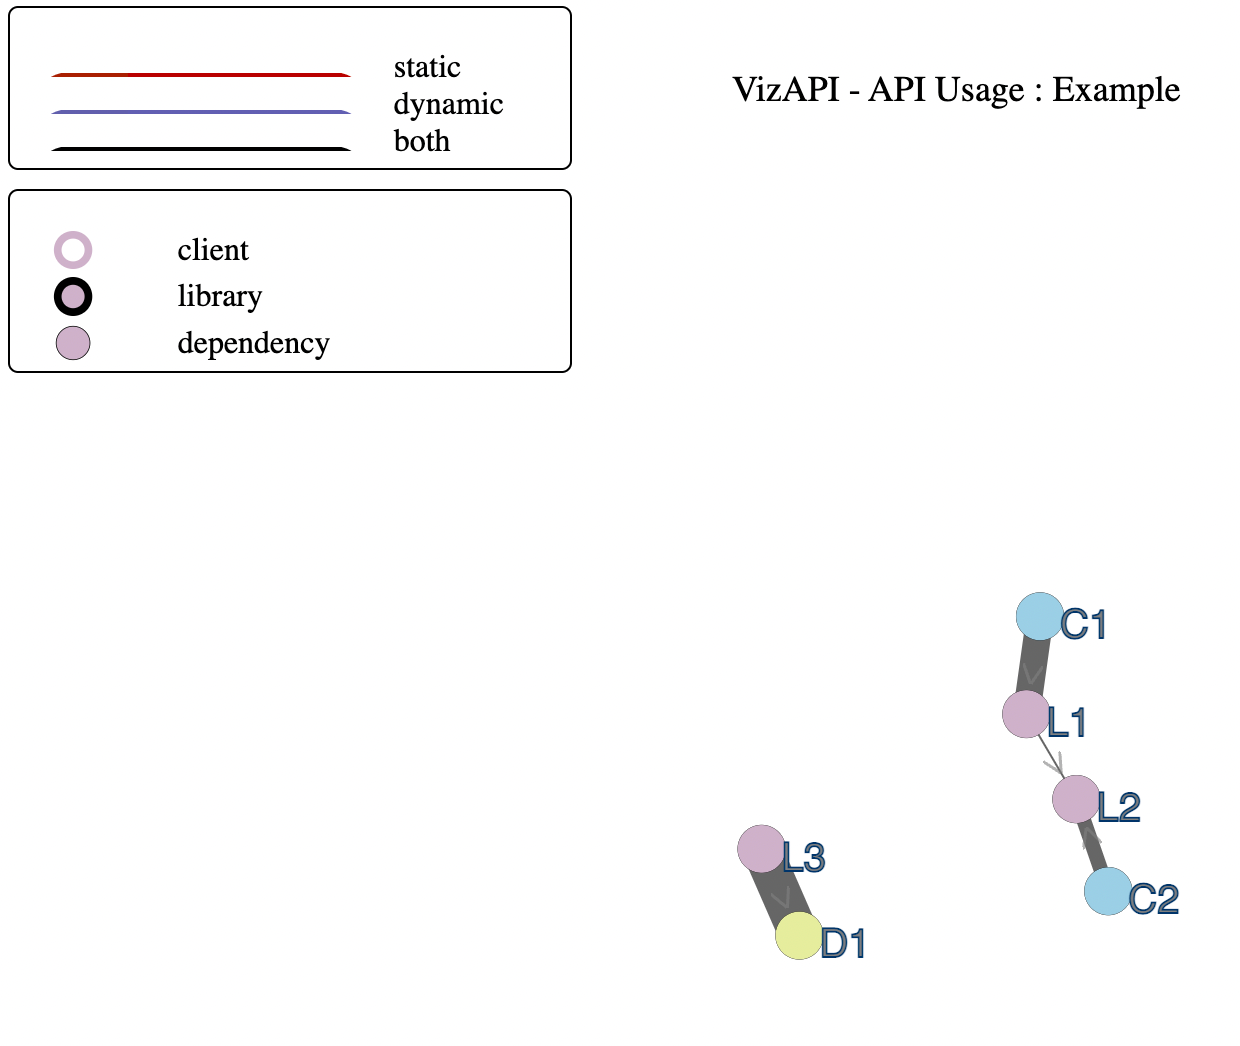
\includegraphics[height=4cm,width=7cm]{images/intro-example.png}
\caption{VizAPI visualization of client C which calls library L, itself dependent on dependency D.}
\label{fig:example}
\end{center}
\end{figure}


Figure~\ref{fig:example} illustrates a VizAPI usage scenario, from the perspective of a client developer. The client is worried about breaking changes in the library. We first define the terms ``client'', ``library'' and ``dependency'', which we use throughout this paper. A `client'' is a software component which directly uses some functionality of an external component, which is the ``library''. Any external component that the ``library'' directly depends on and uses is a ``dependency''. Now consider a client $C$ (blue nodes) and a library $L$ (purple nodes), in the context of plain Java. Library $L$ has packages $L_1$, $L_2$, and $L_3$. $C$ calls into $L_1$ and $L_2$. Internally, within $L$, $L_1$ and $L_2$ call into each other, but not into $L_3$. The VizAPI result, with no edges from $C$ directly to $L_3$, allows a developer to conclude that breaking changes in $L_3$ will not affect $C$. Also, if only $L_3$ uses an external dependency $D$ (yellow node), then we know that $C$ will not need $D$ to be on its classpath.

From the library developer side, under plain Java (i.e. no runtime containers) and considering reflection, the potential API surface of any component is huge. Essentially: every method can be called, and every field can be read and written. Even considering only the published API surface (methods, fields, classes, and annotations with the correct visibility modifiers), libraries' API surfaces still often have hundreds to thousands of members. The breadth of the API surface is a liability with respect to continued maintenance of the library; many developers aspire to avoid breaking changes by preserving, whenever possible, library behaviour that is depended on by clients. Knowing that few clients use a particular API would be valuable.

On the other hand, we would expect (and have verified in our unpublished work) that each client uses only a small portion of each of its dependencies' API surfaces. Consider breaking changes again. GitHub provides the Dependabot tool~\cite{mullans20:_keep_depen}, which monitors for upstream changes and automatically proposes pull requests to update dependency versions. That tool may well pull in breaking changes. However, we hypothesize that, most of the time, most breaking changes will not affect most clients; it is useful for clients to know whether they are using the parts of the API surface that are subject to a particular breaking change. A client with broad dependencies on a library (uses a larger fraction of its API surface) is more likely to be affected by its changes than a client with narrow dependencies (smaller fraction). A narrow library dependency would also suggest that it would be easier to swap the library for a functionally similar replacement.

Additionally, as researchers, we would like to understand how library
APIs are used by clients more generally. Zhong and
Mei~\cite{zhong19:_empir_study_api_usages} investigated API usages in
a dataset of 7 experimental subjects (clients) and the libraries that
they depend on.  They found that clients use less than 10\% of the
declared APIs in libraries. Our visualization allows developers and
researchers to visualize distribution information about how different
parts of clients use different parts of libraries.

This paper presents the VizAPI tool, which shows visualization overviews showing API usages---from clients to libraries, but also between libraries (including transitive dependencies). The goal of VizAPI is to provide a heuristic for developers considering the impacts of changes to libraries. VizAPI incorporates information from static and dynamic analyses.  We have made VizAPI publicly available\footnote{\url{https://github.com/SruthiVenkat/api-visualization-tool}}, although it is still in development. The contributions of this paper include:

% CRAIG emphaised the contributions here

\begin{itemize}

\item \emph{VizAPI}, a tool which presents visualization of API usage information; VizAPI collects static information and instruments Java code and collect dynamic instrumentation information about API uses in practice and presents it as a d3 visualization (Section~\ref{subsec:collecting-data}--\ref{subsec:vis-system});
\item \emph{Case Study}, a discussion of VizAPI usage scenarios (Section~\ref{subsec:evaluation}) based on a collection of 11 libraries and 38 clients.
\end{itemize}


%VizAPI usage scenarios, which we discuss in Section~\ref{sec:discussion}, include guidance to API designers, based on the fact that API usages are sparse, as well as suggestions for tool designers.

%To expand on our aims, we aim to characterize (1) API uses of libraries that are not anticipated by the library developers (``mis-uses'') as well as (2) the empirical extent of API uses by their clients (``API surfaces''). 

%% {\bf Findings.} Our results indicate that API mis-uses are generally rare: developers respect modularity declarations and seldom use reflection to bypass access modifiers (with serialization as a key exception). On the other hand, clients use widely varying portions of their libraries.



%% As a second problem, consider the detection of vulnerabilities in dependencies. Detection is relatively straight-forward: compute the transitive closure of all dependencies, and cross-reference the transitive dependencies with vulnerability databases like CVEs. Tools like \textit{snyk} and \textit{dependabot} are based on this general idea. Some languages and build systems like npm have built-in language-specific support (\textit{npm audit}). The problem is again precision---listing something as a dependency does not mean that all of its functionality is used. So, if dependencies are sufficiently large and deep, a conservative approach inevitably results in false positives. Indeed, Elizalde Zapata et al~\cite{elizalde18:_towar_smoot_librar_migrat} found that 73\% of their studied clients with theoretically vulnerable dependencies were not actually at risk from CVEs in those dependencies, and Chinthanet et al~\cite{chinthanet20:_code_based_vulner_detec_node} implemented a code-based vulnerability detection tool for Node.js applications. Like the boy who cried wolf, false positives can lead to a potentially devastating impact on application security when true positives start being ignored, as demonstrated in the infamous Equifax incident~\cite{luszcz2018apache}. Sadowski et al~\cite{sadowski2018lessons}, among others, also cite the necessity for low false positive rates in developer tools.

%% The basic problem is well-known. In the history of Java (and other languages), several constructs enable component developers to better define and enforce the API surface, including access modifiers, modules, and bundles restricting access to packages, and packaging of components that only expose ``services'', i.e. instantiable classes implementing some abstract type that specifies the service. However, these restrictions always have to compete with the need to provide runtime introspection and code generation features.  Such features are needed to write generic software that can adapt to its usage context. A good example is the automated mapping of domain models to persistency (XML, JSON, RDMBMS, etc).

%  This is often part of another successful trend in modern software engineering---convention over configuration---where services are inferred based on implicit interfaces defined by conventions. 

%In a sense, this has created an arms race:  technologies trying to control APIs versus techniques allowing software to bypass restrictions. This is the space that developers have to navigate when writing modern software.
